%==============================================================================
% Šablona prezentace/Presentation template
% Autoři / Authors: Zdeněk Vašíček, Aleš Smrčka, Jaroslav Dytrych, Jana Stopková, Kristýna Zaklová, Adam Herout
% Kontakt pro dotazy a připomínky: sablona@fit.vutbr.cz
% Contact for questions and comments: sablona@fit.vutbr.cz
%==============================================================================

\documentclass[]{fitthesispresn}

\usepackage[czech, ruled, linesnumbered]{algorithm2e}
\usepackage{algorithmicx}

% Nastavení informací pro úvodní stránku / Setting information for the title page
%---------------------------------------------------------------------------
\projectinfo{
    date=\today, % Datum - je vhodné vepsat datum obhajoby (natvrdo), ne datum kompilace slajdů / Date - it is advisable to write the date of the defense (hard), not the date of the slide compilation        
    title={Cyklická fronta}, % Název prezentace / Presentation title (The whole title of the presented work suitably divided into lines that are optically balanced)
    title.footer={Cyklická fronta}, % Název prezentace - text zobrazovaný vedle čísla slajdu / Presentation title - displayed next to the slide number (The full title of the presented work, it may be suitably abbreviated to fit the footer)
    author.name={Lukáš},  % Jméno autora / Author name
    author.surname={Pšeja}, % Příjmení autora / Author surname
    author.title.first={} % Tituly před jménem autora (jsou-li jaké) / Author's titles before the name (if there are any)
}

% Struktura prezentace / Presentation structure
%---------------------------------------------------------------------------

\begin{document}
    %! UNDERFULL a OVERFULL je bohužel chyba v šabloně, 
    %! psal jsem mail panu doktorovi Jaroslavu Dytrychovi, 
    %! který psal, že to je chyba v šabloně a nemám se tím zabývat, 
    %! takže to prosím neberte jako chybu v mém kódu, děkuji
    \begin{frame}[plain]
        \titlepage
    \end{frame}

    \begin{frame}
        \frametitle{Motivace}
        \begin{itemize}
            \item Cyklická fronta se často využívá v praxi
            \item Je využívána v plánovačích procesů operačních systémů, v síťových systémech při řízení front datových packetů a celkově v systémech, kde je potřeba periodicky zpracovávat události nebo data
            \item \emph{Výhody}\,--\,rychlost, efektivita paměti, využití pro vyrovnávací paměť
            \item \emph{Nevýhody}\,--\,omezená velikost
        \end{itemize}
    \end{frame}

    \begin{frame}
        \frametitle{Co je to cyklická fronta?}
        \begin{columns}
            \column{0.5\textwidth}
            \begin{itemize}
                \item Cyklická fronta je \emph{datová struktura} pro ukládání dat
                \item Je implementovaná jako \emph{zacyklené pole}, což umožňuje \emph{nekonečný} pohyb v poli
                \item Ke správě slouží dva ukazatele, \emph{write} a \emph{read}
                \item Oproti lineárnímu poli je výhodou, že se \emph{nemusí} přesouvat prvky, ale pouze posouvají ukazatele
            \end{itemize}
            \column{0.5\textwidth}
            \begin{figure}[h!]
                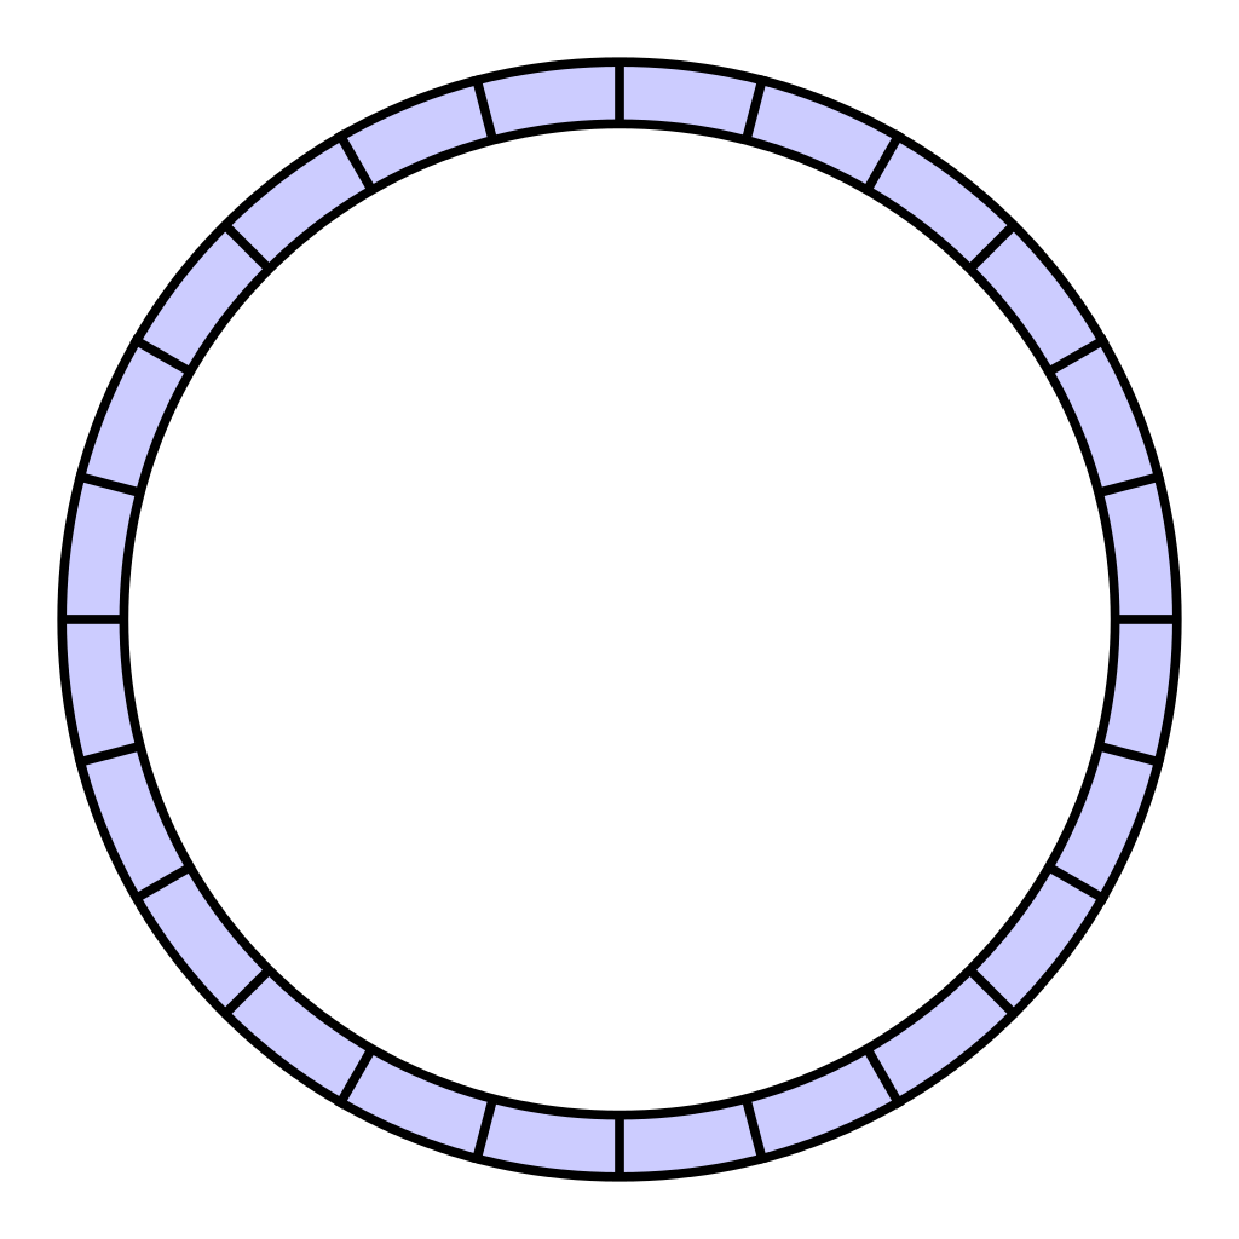
\includegraphics[width=\textwidth]{img/circular_buffer_empty_circle.pdf} % wikipedie - circular buffer
                \caption{Cyklická fronta}
                \label{fig:circular_buffer}
            \end{figure}
        \end{columns}
    \end{frame}

    \begin{frame}
        \frametitle{Struktura cyklické fronty}
        Při implementaci uvažujeme dva způsoby
        \begin{itemize}
            \item Jednodušší způsob, kdy používáme jeden záznam navíc, který nám říká, kolik je momentálně prvků v poli
            \item Složitější ale efektivnější způsob, kdy používáme ukazatele \emph{write} a \emph{read} na výpočet prvků v poli. Aby tato metoda fungovala, musíme ale přidat jeden prvek navíc.
        \end{itemize}
        Druhý způsob je výhodnější, protože je vhodný pro \emph{multithreading} a \emph{real-time} aplikace.

        Jako příklad budeme implementovat UNIXovou funkci \emph{tail}.
        \begin{algorithm}[H]
            \caption{CircularBuffer Struktura}
            \label{alg:circularbuffer}
            \begin{algorithmic}[1]
                \State \textbf{Struktura:} CircularBuffer
                \State \textbf{Prvky:}
                \State \hspace{\algorithmicindent} $\bullet$ \textit{size} : Integer
                \State \hspace{\algorithmicindent} $\bullet$ \textit{head} : Integer
                \State \hspace{\algorithmicindent} $\bullet$ \textit{tail} : Integer
                \State \hspace{\algorithmicindent} $\bullet$ \textit{lines} : Pointer to Pointer to Character
            \end{algorithmic}
        \end{algorithm}
    \end{frame}

    \begin{frame}
        \frametitle{Zakladní operace s cyklickým polem 1/4}
        Kontrola prázdnosti cyklického pole
        \begin{itemize}
            \item Časová složitost kontroly prázdnosti je $O(1)$
        \end{itemize}
        \begin{algorithm}[H]
            \caption{isEmpty}
            \label{alg:isempty}
            \begin{algorithmic}[1]
                \State \textbf{Funkce:} isEmpty
                \State \textbf{Vstup:} CircularBuffer
                \State \textbf{Výstup:} Boolean
                \State \textbf{Pokyny:}
                \State \hspace{\algorithmicindent} \textbf{if} head == tail \textbf{then}
                \State \hspace{\algorithmicindent} \hspace{\algorithmicindent} \textbf{return} True
                \State \hspace{\algorithmicindent} \textbf{else}
                \State \hspace{\algorithmicindent} \hspace{\algorithmicindent} \textbf{return} False
                \State \hspace{\algorithmicindent} \textbf{end if}
            \end{algorithmic}
        \end{algorithm}
    \end{frame}

    \begin{frame}
        \frametitle{Zakladní operace s cyklickým polem 2/4}
        Kontrola plnosti cyklického pole
        \begin{itemize}
            \item Časová složitost kontroly plnosti je $O(1)$
        \end{itemize}
        \begin{algorithm}[H]
            \caption{isFull}
            \label{alg:isfull}
            \begin{algorithmic}[1]
                \State \textbf{Funkce:} isFull
                \State \textbf{Vstup:} CircularBuffer
                \State \textbf{Výstup:} Boolean
                \State \textbf{Pokyny:}
                \State \hspace{\algorithmicindent} \textbf{if} ((tail + 1) \% size) == head; \textbf{then}
                \State \hspace{\algorithmicindent} \hspace{\algorithmicindent} \textbf{return} True
                \State \hspace{\algorithmicindent} \textbf{else}
                \State \hspace{\algorithmicindent} \hspace{\algorithmicindent} \textbf{return} False
                \State \hspace{\algorithmicindent} \textbf{end if}
            \end{algorithmic}
        \end{algorithm}
    \end{frame}

    \begin{frame}
        \frametitle{Zakladní operace s cyklickým polem 3/4}
        Vložení řádku do cyklického pole
        \begin{itemize}
            \item Časová složitost vložení řádku je $O(1)$
        \end{itemize}
        \begin{algorithm}[H]
            \caption{cbufPut}
            \label{alg:cbufPut}
            \begin{algorithmic}[1]
                \State \textbf{Funkce:} cbufPut
                \State \textbf{Vstup:} CircularBuffer, line
                \State \textbf{Pokyny:}
                \State \hspace{\algorithmicindent} \textbf{if} isFull; \textbf{then}
                \State \hspace{\algorithmicindent} \hspace{\algorithmicindent} free(lines[head])
                \State \hspace{\algorithmicindent} \hspace{\algorithmicindent} head = (head + 1) \% size
                \State \hspace{\algorithmicindent} \textbf{else}
                \State \hspace{\algorithmicindent} \hspace{\algorithmicindent}  lines[tail] = line
                \State \hspace{\algorithmicindent} \hspace{\algorithmicindent}  tail = (tail + 1) \% size
                \State \hspace{\algorithmicindent} \textbf{end if}
            \end{algorithmic}
        \end{algorithm}
    \end{frame}

    \begin{frame}
        \frametitle{Zakladní operace s cyklickým polem 4/4}
        Získání řádku z cyklického pole
        \begin{itemize}
            \item Časová složitost získání řádku je $O(1)$
        \end{itemize}
        \begin{algorithm}[H]
            \caption{cbufGet}
            \label{alg:cbufGet}
            \begin{algorithmic}[1]
                \State \textbf{Funkce:} cbufGet
                \State \textbf{Vstup:} CircularBuffer, index
                \State \textbf{Výstup:} Pointer to Character
                \State \textbf{Pokyny:}
                \State \hspace{\algorithmicindent} count = (tail - head + size) \% size
                \State \hspace{\algorithmicindent} \textbf{if} index $<$ 0 \textbf{or} index $\geq$ count; \textbf{then}
                \State \hspace{\algorithmicindent} \hspace{\algorithmicindent} \textbf{return} NULL
                \State \hspace{\algorithmicindent} \textbf{else}
                \State \hspace{\algorithmicindent} \hspace{\algorithmicindent} \textbf{return} lines[(head + index) \% size]
                \State \hspace{\algorithmicindent} \textbf{end if}
            \end{algorithmic}
        \end{algorithm}
    \end{frame}

    \begin{frame}[s]
        \vfill
        \centering \Large Děkuji za pozornost
        \vfill
    \end{frame}

    \begin{frame}
        \frametitle{Zdroje}
        \centering
        \begin{thebibliography}{}
            \bibitem{cbuf} BURNETT, C. (2007, 24. června). Cyklická fronta. Wikipedie [online].\\\url{https://commons.wikimedia.org/wiki/File:Circular_buffer.svg}
            \bibitem{lol} ARPACI-DUSSEAU, Remzi H.; ARPACI-DUSSEAU, Andrea C. (2014).\\Operating Systems: Three Easy Pieces. Arpaci-Dusseau Books. \url{http://pages.cs.wisc.edu/~remzi/OSTEP/}
            \bibitem{pepe} PERINGER, P. Domácí úloha 2. (2024, 26. března).\\ \url{https://www.fit.vutbr.cz/study/courses/IJC/public/DU2.html.cs}
        \end{thebibliography}
    \end{frame}

\end{document}
